\documentclass[10pt,twocolumn]{article}
\usepackage[margin=0.75in]{geometry}
\usepackage{amsmath,amssymb,booktabs,graphicx,adjustbox,caption}
\usepackage[colorlinks=true,urlcolor=blue,citecolor=blue]{hyperref}
\setlength{\parskip}{2pt}

\begin{document}

\title{Supplementary Material for ``GPU-Accelerated Uncertainty Quantification for
Network Congestion: Coupled SDE Simulation and a Systematic Comparison of
Rare-Event Estimators''}
\author{Paritosh Dwivedi and Anindita Kundu}
\date{}
\twocolumn[\begin{@twocolumnfalse}\maketitle\vspace{6mm}\end{@twocolumnfalse}]

\section*{Scope}

This supplement holds material referenced from, but not reproduced in, the main
manuscript. Reviewer~1 asked us to compress the secondary modules; rather than
delete these measurements we moved them here in full, so every number remains
available and auditable. Nothing here is new evidence: each item supports a
conclusion already stated and justified in the main text.

All measurements are on hardware we ran. No projected or modelled performance
value appears in this supplement, consistent with the main manuscript.

\section{Kernel Roofline Characterisation}

\subsubsection{Roofline Analysis}
\label{subsec:roofline}

Figure~\ref{fig:roofline_t4_a100} plots the roofline model for the SDE EM kernel on both
Tesla~T4 and A100 80\,GB PCIe (FP32).  Operational intensity is computed from the dominant
operation---a dense $(N_p{\times}n)\times(n{\times}n_{\mathrm{local}})$ matrix--vector
multiply per EM step---giving
$\mathrm{OI}=(2N_pn^2+6N_pn)\,/\,(4(N_pn+n^2+2N_pn))$\,FLOPs/byte,
which ranges from 50--196 across the evaluated sizes.

The two devices have very different ridge OIs (T4: 25.4; A100: 161\,FLOPs/byte), placing
the same kernel in different regimes on each device (Table~\ref{tab:roofline}).
On T4, whose lower ridge reflects its modest memory bandwidth (320\,GB/s), all three sizes
land \emph{above} the ridge: the kernel is \textbf{compute-bound}, and efficiency climbs
from 14\% ($n{=}500$) to 49\% ($n{=}5{,}000$).  On A100, with its 1935\,GB/s bandwidth and
312\,TFLOPS FP32 peak, the ridge sits at 161\,FLOPs/byte: $n{=}500$ falls below it
(memory-bound, 0.8\%) and $n{=}5{,}000$ reaches the transitional zone (5.0\%).  In both
cases GPU utilisation grows monotonically with $n$, directly explaining why larger graph sizes
benefit disproportionately from GPU execution and validating the workload-saturation story: at
small~$n$ the SDE EM kernel is overhead- or bandwidth-limited; at $n{\gtrsim}5{,}000$ it
approaches the compute roofline on T4 and enters the transitional zone on A100.



\begin{table}[!t]
\caption{Roofline characterisation of the SDE EM kernel on T4 and A100 (FP32,
512 paths, 100--200 steps). OI = FLOPs/Byte. Ridge OI: T4\,=\,25.4; A100\,=\,161.}
\label{tab:roofline}
\centering\small
\resizebox{\columnwidth}{!}{%
\begin{tabular}{@{}l r r r r l@{}}
\toprule
Device & $n$ & OI (FLOPs/B) & Achieved (GFLOPs/s) & Efficiency & Bound \\
\midrule
T4  & 500   &  63.2 & 1{,}137  & 14.0\% & compute \\
T4  & 1{,}000 & 101.2 & 2{,}240  & 27.5\% & compute \\
T4  & 5{,}000 & 196.0 & 3{,}967  & 48.7\% & compute \\
\midrule
A100 & 500   &  50.5 & 2{,}528  &  0.8\% & memory \\
A100 & 1{,}000 &  84.2 & 8{,}567  &  2.7\% & transitional \\
A100 & 5{,}000 & 181.7 & 15{,}742 &  5.0\% & transitional \\
\bottomrule
\end{tabular}}
\end{table}

\begin{figure}[!t]
\centering
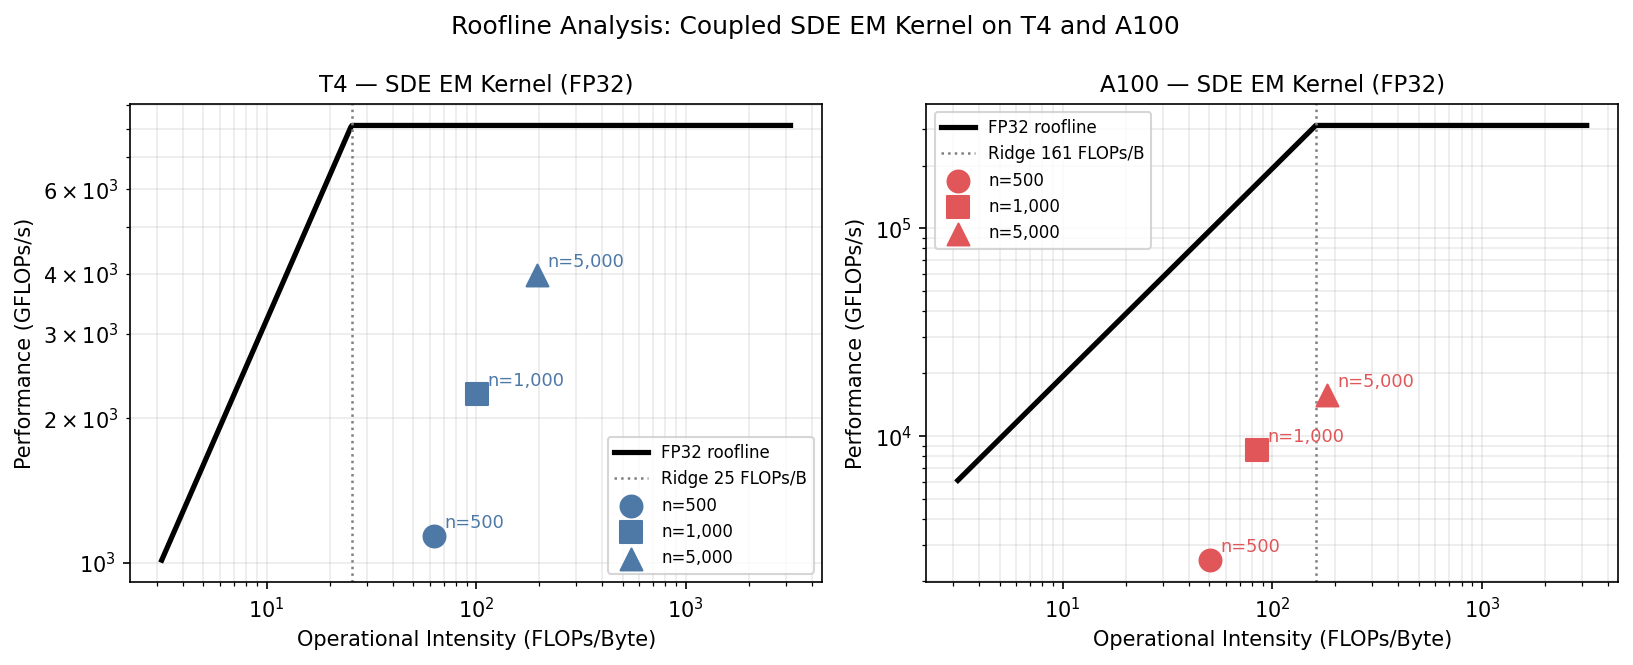
\includegraphics[width=0.95\columnwidth]{roofline_T4_A100.png}
\caption{Roofline model for the SDE EM kernel on T4 (left, ridge 25\,FLOPs/B) and
A100 (right, ridge 161\,FLOPs/B). Points move right and up with $n$, indicating
growing compute intensity and efficiency. T4 kernels are compute-bound across all sizes;
A100 kernels are memory-bound at $n{=}500$ and transitional by $n{=}5{,}000$.
Both devices confirm the same trend: GPU utilisation recovers as workload grows.}
\label{fig:roofline_t4_a100}
\end{figure}

\section{Single-GPU Kernel Phase Breakdown}

Table~\ref{tab:phase_breakdown} gives the \texttt{torch.profiler} phase decomposition of one
fine-level path loop referenced from the main text, measured on a Tesla~T4 over three seeds by
device-side (CUPTI) kernel time. The degenerate single-rank all-reduce phase is omitted, as it
measures nothing communicable and is not part of the single-GPU cost. The trend is that kernel
launch/dispatch dominates at small graph size and the drift matrix multiply overtakes it as the
kernels grow, while the Skorokhod reflection and the multilevel bookkeeping remain negligible
throughout---so the reflected-boundary treatment and the telescoping sum, the two
problem-specific additions, cost almost nothing. The two dominant kernels at $n{=}5{,}000$ are
\texttt{aten::mm} and the underlying \texttt{sgemm} (the drift matmul), each $\approx$19\,ms per
loop; every elementwise kernel (reflection clamp, noise scaling, level differencing) is under
0.25\,ms combined.

A measured peak-memory pass in the same run shows the manuscript's adjacency-only memory model
($n^2$ bytes at single precision) is accurate only once the adjacency dominates: at $n{=}500$ the
true allocator peak is $13.6\times$ the model (fixed ensemble and predictor--corrector buffers
the model omits), but by $n{=}5{,}000$ the ratio is $1.10\times$, confirming the model as a valid
large-$n$ scaling driver rather than an absolute figure. Achieved SM occupancy is not reported:
it requires Nsight Compute (\texttt{ncu}), which the CUPTI trace does not expose, and we do not
estimate it.

\begin{table}[!t]
\caption{Single-GPU phase breakdown of one fine-level path loop (Tesla~T4, three seeds, mean
percentage of traced device-side kernel time). All values MEASURED. Raw per-seed data in
\texttt{results/profiling\_gpu/}.}
\label{tab:phase_breakdown}
\centering\small
\begin{tabular}{@{}l r r@{}}
\toprule
Phase & $n{=}500$ (\%) & $n{=}5{,}000$ (\%) \\
\midrule
Kernel launch / dispatch     & 65.3 & 50.5 \\
Drift matrix multiply        & 27.6 & 48.9 \\
Random-number generation     & 5.0  & 0.4  \\
Skorokhod reflection         & 1.4  & 0.2  \\
MLMC level bookkeeping       & 0.7  & 0.1  \\
\bottomrule
\end{tabular}
\vspace{2pt}
\footnotesize Measured peak memory (same run): $n{=}500$, 13.6\,MB ($13.6\times$ the
adjacency-only model); $n{=}5{,}000$, 109.8\,MB ($1.10\times$ the model).
\end{table}

\section{Multi-GPU Measurements}

The main text reports the multi-GPU contribution as \emph{memory scalability}
rather than strong-scaling speedup, and gives the headline weak- and
strong-scaling figures. The per-configuration measurements behind those
statements are collected here.

\begin{table}[!t]
\caption{4-GPU weak-scaling at large $n$ on 4$\times$RTX\,3090 PCIe ($\varepsilon{=}0.05$).
Single-GPU reference from A100 80\,GB PCIe (Table~\ref{tab:large_scale}); efficiency is a
conservative bound due to device-generation difference. Efficiency recovers monotonically
with $n$, confirming PCIe all-reduce amortisation at large workloads.}
\label{tab:multigpu_4gpu}
\centering\small
\resizebox{\columnwidth}{!}{%
\begin{tabular}{@{}r r r r r@{}}
\toprule
$n$ & 1-GPU A100 (s) & 4-GPU 3090 (s) & Mem/GPU (MB) & Eff.\ (bound) \\
\midrule
5{,}000  & 0.117 & 0.124 & 262      & 24\% \\
10{,}000 & 0.296 & 0.212 & 973      & 35\% \\
25{,}000 & 1.443 & 0.731 & 5{,}816  & 49\% \\
\bottomrule
\end{tabular}}
\end{table}

\begin{table}[!t]
\caption{Compute vs.\ Communication Breakdown on 4$\times$RTX\,3090 (PCIe, $n{=}1000$,
weak-scaling configuration). All-reduce time measured via NCCL event timing; compute time
is total wall time minus all-reduce. The 43\% efficiency at $G{=}4$ is entirely
communication-bound: compute time is flat across world sizes.}
\label{tab:comm_breakdown}
\centering
\resizebox{\columnwidth}{!}{%
\begin{tabular}{@{}r r r r r r@{}}
\toprule
GPUs & Compute (ms) & All-reduce (ms) & Total (ms) & Comm \% & Efficiency \\
\midrule
1 &  75 &   0 &  75 &  0.0\% & 100\% \\
2 &  75 &   1 &  76 &  1.3\% &  99\% \\
4 &  65 & 110 & 175 & 62.9\% &  43\% \\
\bottomrule
\end{tabular}}
\end{table}

\begin{table}[!t]
\caption{Blocking vs.\ overlapped NCCL all-reduce at $G{=}2$ and $G{=}4$
($n{=}2{,}000$, $\varepsilon{=}0.05$, 5 reps, PCIe hardware).
Overlap Gain $= (T_{\mathrm{block}}-T_{\mathrm{overlap}})/T_{\mathrm{block}}$;
Hidden fraction $H = (T_{\mathrm{block}}-T_{\mathrm{overlap}})/T_{\mathrm{allreduce}}$.
The larger all-reduce payload at $G{=}4$ (more processes) increases the absolute gain.}
\label{tab:overlap}
\centering\small
\resizebox{\columnwidth}{!}{%
\begin{tabular}{@{}l r r@{}}
\toprule
Metric & $G{=}2$ (RTX\,A5000) & $G{=}4$ (RTX\,3090) \\
\midrule
$T_{\mathrm{block}}$     & $64.2 \pm 2.5$\,ms & $91.3 \pm 2.9$\,ms \\
$T_{\mathrm{overlap}}$   & $57.4 \pm 0.3$\,ms & $74.6 \pm 1.9$\,ms \\
$T_{\mathrm{allreduce}}$ & $11.5$\,ms         & $30.5$\,ms \\
Overlap Gain             & $10.6\%$            & $18.3\%$ \\
Hidden fraction $H$      & $59.3\%$            & $54.9\%$ \\
Visible comm             & $4.7$\,ms           & $13.8$\,ms \\
\bottomrule
\end{tabular}}
\end{table}

\section{Halo-Exchange Staleness Sweep}

The halo-exchange interval $K$ trades communication volume against estimator
bias, with the bias bounded by the staleness term
$\mathcal{O}(L_{\mathrm{lip}} K h_\ell)$ derived in the main text. The sweep
below is the measurement supporting the recommended operating point $K{=}2$.

\begin{table}[!t]
\caption{Halo-exchange interval sweep ($G{=}4$ RTX\,3090 PCIe, $n{=}2{,}000$,
$\varepsilon{=}0.05$, 5 seeds). Runtime and bias relative to $K{=}1$ (fully correct
baseline). Phase breakdown shows fraction of wall time per component; Sync\,$\approx$0\%
at all $K$. $K{=}2$ is recommended: 22.5\% runtime reduction at 2.9\% bias.}
\label{tab:halo_sweep}
\centering\small
\resizebox{\columnwidth}{!}{%
\begin{tabular}{@{}r r r r r r r@{}}
\toprule
$K$ & Runtime (ms) & RT Reduc. & Bias & SDE\% & Book.\% & Halo\% \\
\midrule
1 & $94.8\pm6.3$ & ---    & ---    & 51.1\% & 7.2\% & 41.7\% \\
2 & $73.5\pm4.0$ & 22.5\% &  2.9\% & 68.5\% & 8.0\% & 23.5\% \\
4 & $58.7\pm3.7$ & 38.1\% &  7.9\% & 77.9\% & 9.3\% & 12.8\% \\
8 & $51.5\pm1.3$ & 45.7\% & 15.3\% & 83.0\% & 10.0\% &  7.0\% \\
\bottomrule
\end{tabular}}
\end{table}

\begin{figure}[!t]
\centering
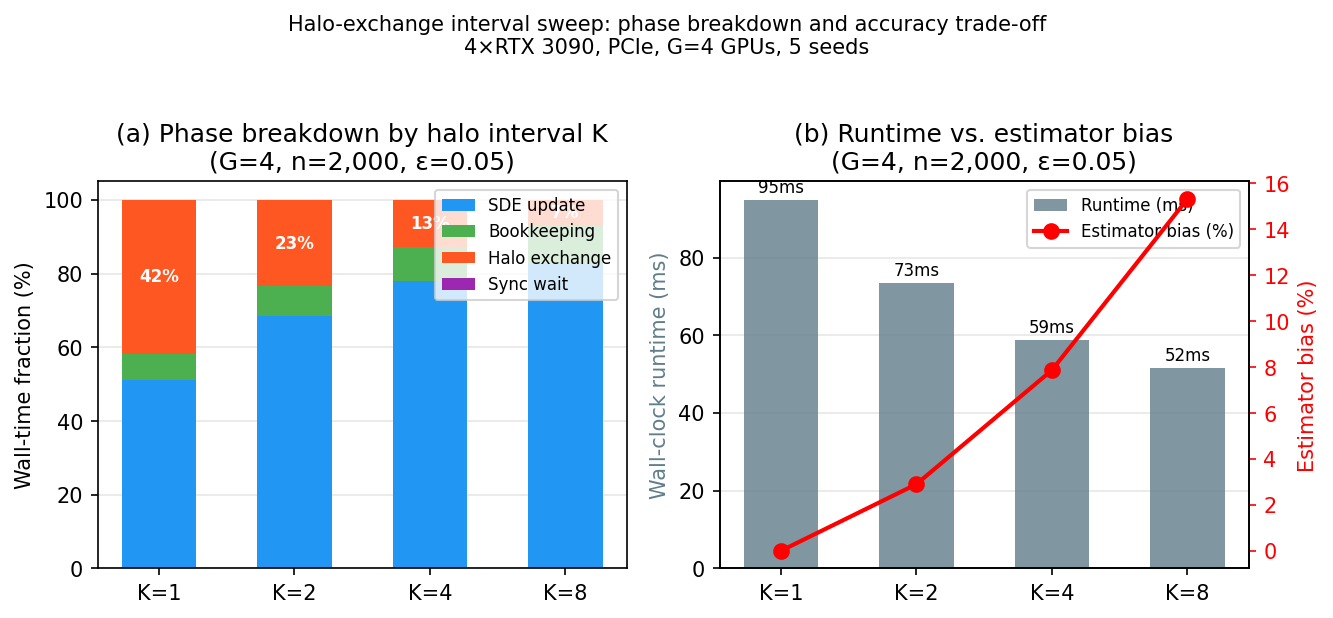
\includegraphics[width=0.98\columnwidth]{halo_phase_breakdown.png}
\caption{Halo-exchange interval sweep ($G{=}4$ RTX\,3090 PCIe, $n{=}2{,}000$,
$\varepsilon{=}0.05$, 5 seeds).
\emph{Left:} stacked phase breakdown showing the fraction of wall time in each component
(SDE update, MLMC bookkeeping, halo/all-reduce, sync wait) for $K{=}1,2,4,8$.
At $K{=}1$ the halo phase accounts for 41.7\% of total runtime; $K{=}2$ halves this to 23.5\%,
proportionally increasing SDE compute time.
\emph{Right:} runtime (bars) and estimator bias (red line) as functions of $K$, showing the
accuracy--efficiency trade-off. $K{=}2$ offers 22.5\% runtime reduction at only 2.9\% bias.}
\label{fig:halo_phase}
\end{figure}

\section{Data Availability}

Every table in this supplement is reproduced by the scripts in the accompanying
repository under \texttt{scripts/}, writing to \texttt{results/}. The
per-seed raw data for the main manuscript's evidence tables is archived under
\texttt{results/baselines/}, \texttt{results/topology\_matrix/},
\texttt{results/topology\_matrix\_stress/}, \texttt{results/validity\_envelope/},
\texttt{results/rare\_event\_comparators/} and \texttt{results/significance/}.

\end{document}
